\subsection{Practice Problems}
\begin{enumerate}
    \item What is the change in entropy of a system undergoing an adiabatic\footnote{For anyone going on to take 203, in this question we would also technically have the qualifier that the process was also \textbf{quasistatic}, but this is not relevant for our discussion here!} process? (Hint: return to the classical definition).
    \item Consider a situation where you are determining the entropy of rolling three (unique/distinguishable) dice. Consider the macrostate $7$, where $7$ is the sum of the three dice. What is the entropy of this macrostate?
    \item How does the answer to the above question change if you consider three indistinguishable dice? In this case, (1,1,2) and (1,2,1) would be the same, for example.
    \item What is the change in entropy of the gas medium of \textbf{any} heat engine after one cycle? Why?
    \item Explain using macrostates/microstates why if I remove a partition between two different gases in a box, why they will mix irreversibly and will never return to their original state. 
    \item Suppose I have a one mole of monoatomic gas of volume $V = 1m^3$ and temperature $T = 300K$. I first (isochorically) heat it up to $T=400K$, then I let it expand isothermally so that it is double its original size. What is the change in entropy of the gas (Hint: Use equation 34)?
    \item Imagine we have two compartments of gas separated by a movable piston (that is initially locked in place), initially located in the center. The two containers cannot exchange heat with each other (nor with their surroundings), and have the same initial volume $V$ and amount of gas $n$. Now assume that, initially, the temperature of the gas in the piston on the right hand side ($T_R$) is higher than that on the left ($T_L$). 
    \begin{enumerate}
        \item When I unlock the piston, what happens?
        \item What is the change in internal energy and entropy of the whole system?
        \item What can you say of the pressure, volume, and temperature on both sides at the end? Will the system be at thermal equilibrium?
    \end{enumerate}  
    
    \begin{center}
        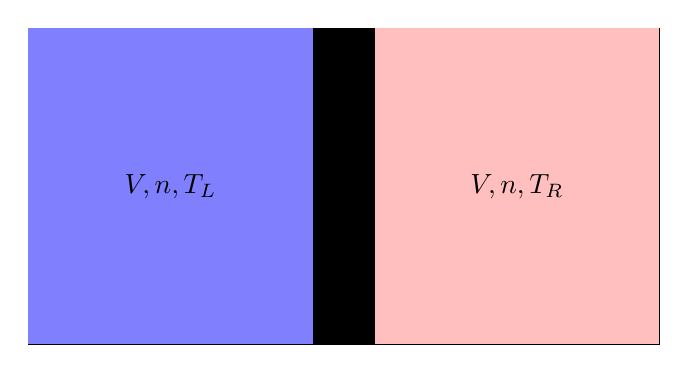
\begin{tikzpicture}[scale=4]
        \draw[black, thick] (0,0) rectangle (2,1);
        \filldraw[fill = black, draw = black] (0.9,0) rectangle (1.1,1);
        \filldraw[fill = blue!50, draw = blue!50] (0,0) rectangle(0.9,1);
         \filldraw[fill = pink, draw = pink] (1.1,0) rectangle(2,1);
        \draw[black] (0.45,0.5) node {$V,n,T_L$};
        \draw[black] (1.55,0.5) node {$V,n,T_R$};
        
        \end{tikzpicture}
    \end{center}
\end{enumerate}